\documentclass[a4paper,12pt]{article}
\usepackage[paperwidth=210mm,paperheight=297mm,left=27mm,right=27mm,top=27mm,bottom=27mm]{geometry}

\usepackage{graphicx}
\usepackage{blindtext}
\usepackage{adjustbox}
\usepackage{natbib}
\usepackage{lipsum}

\usepackage{bibentry}

\bibliographystyle{jmr}

\title{EEGS - Introduction to Stata\thanks{Escola de Economia e Gestão, Universidade do Minho, Portugal}}
\date{May, 2021}
\author{Anabela Carneiro\\ U Porto
\and João Cerejeira \\ U Minho
\and Miguel Portela \\ U Minho 
\and Paulo Guimarães \\ Banco de Portugal \& U Porto}

\begin{document}

\maketitle

\section{Introduction}\label{sec:intro}

Figure \ref{fig:incdensity} sets the stage for our example, while Table \ref{tb:descriptives} shows descriptive statistics for the data used in the regression analysis. It shows a kerndel density for income. Table \ref{tb:regresults} presents our regressions. One could follow the book by \cite{acemoglu2016} to motivate the discussion. A thorough discussion of Econometrics is provided by \cite{greene2017} (see also \citep{verbeek2012}).\footnote{\cite{wooldridge2015introductory} makes a good introduction to Econometrics.}

\lipsum

\begin{table}[h]
\begin{center}
\caption{Descriptive statistics}\label{tb:descriptives}
\resizebox{0.9\textwidth}{!}
	{\begin{tabular}{lcccccc} \hline
VARIABLES & N & Mean & P99 & s.d. & Min & Max \\ \hline
Real GDP per worker & 857 & 19,902 & 74,706 & 21,470 & 396 & 271,192 \\
Education (in years) & 857 & 4.77 & 11.43 & 2.88 & 0.04 & 12.25 \\
Capital & 234 & 5,498 & 1,021 & 1,582 & 1,195 & 1,121 \\
Degree of openness & 857 & 62.86 & 290.20 & 52.18 & 2.32 & 395.98 \\ \hline
\end{tabular}}
\end{center}
\end{table}

\begin{figure}[ht]
	\begin{center}
		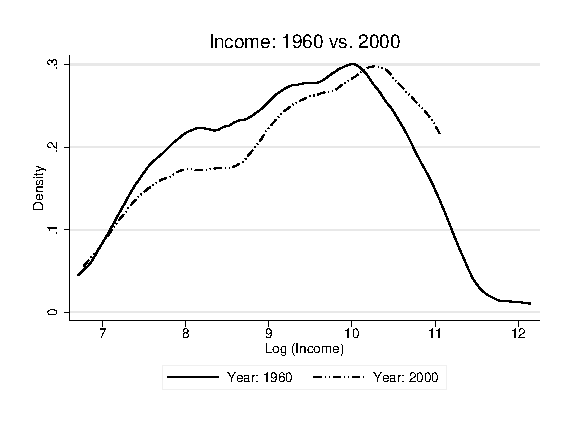
\includegraphics[scale = 0.5,trim = 0.0 0.0 0.0 0.0,clip]{income_density.eps}
		\caption{Income density}\label{fig:incdensity}
	\end{center}
\end{figure}

\begin{table}[ht]
\caption{Regression analysis}\label{tb:regresults}
	\begin{center}
		\begin{center}
\begin{tabular}{lc}
\hline \noalign{\smallskip} & Simple model\\
\noalign{\smallskip}\hline \noalign{\smallskip}Education & 0.3169***\\
 & \begin{footnotesize}(0.0093)\end{footnotesize}\\
\noalign{\smallskip}Capital & \\
\noalign{\smallskip}Openness degree & \\
\noalign{\smallskip}$R^2$ & 0.58\\
RMSE & 0.78\\
$N$ & 857\\
\noalign{\smallskip}\hline\end{tabular}\\
\smallskip\begin{footnotesize}\ * $p<0$.1; ** $p<0$.05; *** $p<0$.01\end{footnotesize}\\
\smallskip
\end{center}

	\end{center}
\end{table}

\bibliography{references}

\end{document}
